\section{Rewards and collectables}
One of the main components to Sophie's Flying Castle game is finding collectibles throughout the world.
Collectibles are items that are required to be collected in order to achieve 100\%
completion of the game, but they are not compulsorily required to go on in the main storyline. Collectibles, along with coins and crafting materials, are the fundamental part of the reward system of the game; in fact they constitute the prizes for any successful in-game action of the player. Moreover they even grant rewards to all the players who will deeply explore the maps, reaching high percentages of completion of the game.\\

There are three category of collectibles:
\begin{enumerate}
\item \textbf{Hats}: these objects can be hats, wigs and helmets. If they are worn they provide skill bonus during the game wherever Sophie is as long as she keeps them on.
\item \textbf{Lanterns}: these objects work as weapons for Sophie. They contain Calcifer and they are evolutions of the basic lantern, given to Sophie at the beginning of the story. While they are held by Sophie, they provide skill bonus during the combat against enemies. 
\item \textbf{Clothes}: these object are special clothes that Sophie may get during the game and they provide effect depending on where Sophie is.  
  \end{enumerate}

Generally speaking, a player can only use one object per category at a time.

Example: if Sophie had unlocked two or more magic hats, she could still wear only one. But if she had unlocked also a magic lantern, she might wear a hat and hold the lantern.
Collectables can be sold for Difficulty * 10 coins at merchants' stands, crafting materials can be sold for half of their buying price at merchants' stands.
\subsection{Level completion rewards}
These collectables are items that Sophie is granted to receive after completing a level.

%These are tied to a small reward in coins, materials or experience and bound to levels of Sophie's abilities.

%The player will receive these items just by playing the main story of the game.\\\\
There are three category of rewards:
\begin{enumerate}
\item \textbf{Hats}\\
  \begin{longtable}[H]{|p{2cm}|p{1.5cm}|p{2cm}|p{2.8cm}|p{6.3cm}|}
\hline
\multicolumn{5}{|c|}{\cellcolor[HTML]{656565}{\color[HTML]{FFFFFF} \textbf{Collectable}}}                                                                                                                                                                                                                                                                                                                                \\ \hline
\multicolumn{1}{c|}{\cellcolor[HTML]{C0C0C0}\textbf{Hats}} & \cellcolor[HTML]{C0C0C0}{\color[HTML]{000000} \textbf{Image}} & \multicolumn{1}{c|}{\cellcolor[HTML]{C0C0C0}{\color[HTML]{000000} \textbf{Level}}} & \multicolumn{1}{c|}{\cellcolor[HTML]{C0C0C0}{\color[HTML]{000000} \textbf{Bonus}}}   & \multicolumn{1}{c|}{\cellcolor[HTML]{C0C0C0}{\color[HTML]{000000} \textbf{Brief description}}}                                        \\ \hline
\textbf{Derby}                       & \raisebox{-0.3\height}{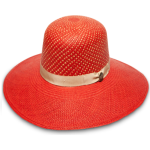
\includegraphics[height=1.5cm]{Images/Hats/derby}}              & First Steps                                                                        & +1 Intelligence                                                                      & Sophie is getting it in a tutorial level where she learns how to sew new hats.                                                        \\ \hline
\textbf{A}                           & AA                                                            & Where is Howl                                                                      & AAA                                                                                  & AAAA                                                                                                                                  \\ \hline
\textbf{B}                           & BB                                                            & The imprisoned friend                                                              & BBB                                                                                  & BBBB                                                                                                                                  \\ \hline
\textbf{C}                           & CC                                                            & Nasty surprise(s)                                                                  & CCC                                                                                  & CCCC                                                                                                                                  \\ \hline
\textbf{D}                           & DD                                                            & Battle cry                                                                         & DDD                                                                                  & DDDD                                                                                                                                  \\ \hline
\textbf{E}                           & EE                                                            & An ancient legend                                                                  & EEE                                                                                  & EEEEE                                                                                                                                 \\ \hline
\textbf{F}                           & FF                                                            & The djiin of the desert                                                            & FFF                                                                                  & FFFFF                                                                                                                                 \\ \hline
\textbf{Bue hair}                    & \raisebox{-0.3\height}{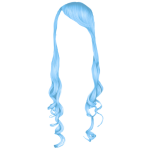
\includegraphics[height=1.5cm]{Images/Hats/blueHair}}           & Nel blu dipinto di blu                                                             &                                                                                      & Sophie is getting it in when she begins to drive the castle.                                                                          \\ \hline
\textbf{Desert}                      & \raisebox{-0.3\height}{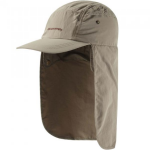
\includegraphics[height=1.5cm]{Images/Hats/desert}}             & The last hope                                                                      & \begin{tabular}[c]{@{}l@{}}+3 HP\\ +1 Consitution\\ -1 AC\\ -1 Charisma\end{tabular} &                                                                                                                                       \\ \hline
\textbf{G}                           & GG                                                            & The spirits realm                                                                  & GGG                                                                                  & GGGG                                                                                                                                  \\ \hline
\textbf{H}                           & HH                                                            & Fire and secrets                                                                   & HHH                                                                                  & HHHH                                                                                                                                  \\ \hline
\textbf{I}                           & II                                                            & Mizar's past                                                                       & III                                                                                  & IIIII                                                                                                                                 \\ \hline
\textbf{L}                           & LL                                                            & The final choice                                                                   & LLL                                                                                  & is a trophy that Sophie can get if She chooces to spare Mizar. Sophie keeps this hat in her bags if she start the game a second time  \\ \hline
\textbf{M}         
  \end{longtable}

\item \textbf{Lanterns}\\
  \begin{longtable}[H]{|p{2cm}|p{1.5cm}|p{2cm}|p{2.8cm}|p{6.3cm}|}
\multicolumn{5}{|c|}{\cellcolor[HTML]{656565}{\color[HTML]{FFFFFF} \textbf{Collectable}}}                                                                                                                                                                                                                                                                                                                                            \\ \hline
\multicolumn{1}{c|}{\cellcolor[HTML]{C0C0C0}\textbf{Lanterns}} & \cellcolor[HTML]{C0C0C0}{\color[HTML]{000000} \textbf{Image}}                               & \multicolumn{1}{c|}{\cellcolor[HTML]{C0C0C0}{\color[HTML]{000000} \textbf{Level}}} & \multicolumn{1}{c|}{\cellcolor[HTML]{C0C0C0}{\color[HTML]{000000} \textbf{Bonus}}} & \multicolumn{1}{c|}{\cellcolor[HTML]{C0C0C0}{\color[HTML]{000000} \textbf{Brief description}}}                     \\ \hline
%\textbf{} & \multicolumn{1}{c|}{} & First Steps &  &  \\ \hline
\textbf{Magic lantern} & \raisebox{-0.3\height}{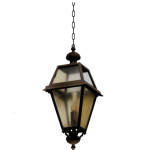
\includegraphics[height=1.5cm]{Images/Lanterns/basis}}
& Where is Howl? & No bonus  & Sophie is getting it before leaving to Dynamia. This is the basis weapon of Sophie. \\ \hline
\textbf{Demonic} & \raisebox{-0.3\height}{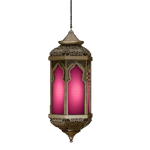
\includegraphics[height=1.5cm]{Images/Lanterns/demonic}} & The imprisoned friend
& TODO & Sophie will get it before just if She chooses to fight the prisons boss in the castle of Dynamia and defeat him.   \\ \hline
%\textbf{} & & Nasty surprise(s) &  & \\ \hline
%\textbf{}  &  & Battle cry & & \\ \hline
%\textbf{} & & An ancient legend & &  \\ \hline
%\textbf{} &  & The djiin of the desert & & \\ \hline
%\textbf{} & & Nel blu dipinto di blu &  & \\ \hline
\textbf{Belzel's lantern} & \raisebox{-0.3\height}{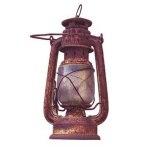
\includegraphics[height=1.5cm]{Images/Lanterns/belzel}} & The last hope & TODO  & Sophie may get Belzel's lantern just completing a seconday mission given from Belzel. \\ \hline
%\textbf{} &  & The spirits realm & & \\ \hline
%\textbf{} & & Fire and secrets & & \\ \hline
\textbf{Gold} & \raisebox{-0.3\height}{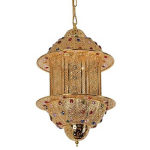
\includegraphics[height=1.5cm]{Images/Lanterns/gold}} & Mizar's past & TODO &
Sophie is getting it together the Mizar's heart. \\ \hline
\textbf{Five Hits} & \raisebox{-0.3\height}{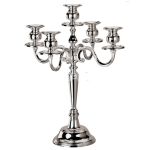
\includegraphics[height=1.5cm]{Images/Lanterns/candelabrumFiveHits}} &
The final choice  & +5 Strength & Sophie can get if She chooces to spare Mizar. Sophie keeps it in her bags if she start the game a second time      \\ \hline
\textbf{Cristal} & \raisebox{-0.3\height}{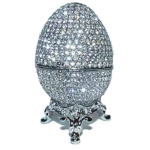
\includegraphics[height=1.5cm]{Images/Lanterns/cristal}} & The final choice
& TODO & Sophie can get if She chooces to defeat Mizar. Sophie keeps it hat in her bags if she start the game a second time \\ \hline
\end{longtable}

\item \textbf{Clothes}\\
  \begin{longtable}[H]{|p{2cm}|p{1.5cm}|p{2cm}|p{2.8cm}|p{6.3cm}|}
\hline
\multicolumn{5}{|c|}{\cellcolor[HTML]{656565}{\color[HTML]{FFFFFF} \textbf{Collectable}}}                                                                                                                                                                                                                                                                                                              \\ \hline
\multicolumn{1}{c|}{\cellcolor[HTML]{C0C0C0}\textbf{Clothes}} & \cellcolor[HTML]{C0C0C0}{\color[HTML]{000000} \textbf{Image}} & \multicolumn{1}{c|}{\cellcolor[HTML]{C0C0C0}\textbf{Levels}} & \multicolumn{1}{c|}{\cellcolor[HTML]{C0C0C0}{\color[HTML]{000000} \textbf{Bonus}}}    & \multicolumn{1}{c|}{\cellcolor[HTML]{C0C0C0}{\color[HTML]{000000} \textbf{Brief description}}}                                         \\ \hline
\textbf{Sophie's dress}& \raisebox{-0.8\height}{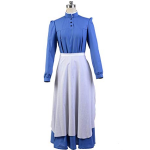
\includegraphics[height=1.5cm]{Images/Clothes/sophie}} & First steps & No bonus
& This is the Sophie's basic dress. \\ \hline
\textbf{Guard}& \raisebox{-0.8\height}{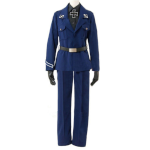
\includegraphics[height=1.5cm]{Images/Clothes/guards}} & The imprisoned friend & If the guards of Dynamia haven’t yet seen her, they take longer to spot her in Dynamia while
they are next to her. & Sophie can get it from a secondary mission in the castle of Dynamia. She can follow a guard until he reaches a locker
room and take his clothes when he is gone. \\ \hline

\end{longtable}


\end{enumerate}


\subsection{Others collectables and trophies}
These collectables are not story-dependent and the player could get them at anytime during the game. They are tided to a medium/big reward in coins, materials or experience, but still bound to levels of Sophie's abilities. In order to receive them the player has to play the game deeply, exploring areas outside the ones he encountered during the main story flow, investing more time to get higher rewards.
\begin{enumerate}
\item \textbf{Hats}\\
  {\small
\begin{longtable}[H]{|p{1.8cm}|p{1.5cm}|p{2cm}|p{2.6cm}|p{5.3cm}|p{1.2cm}|}
\hline
\multicolumn{6}{|c|}{\cellcolor[HTML]{656565}{\color[HTML]{FFFFFF} \textbf{Collectable}}} \\\hline
\multicolumn{1}{c|}{\cellcolor[HTML]{C0C0C0}\textbf{Hats}} & \cellcolor[HTML]{C0C0C0}{\color[HTML]{000000} \textbf{Image}} &
\multicolumn{1}{c|}{\cellcolor[HTML]{C0C0C0}\textbf{Location}} &
\multicolumn{1}{c|}{\cellcolor[HTML]{C0C0C0}{\color[HTML]{000000} \textbf{Bonus}}} &
\multicolumn{1}{c|}{\cellcolor[HTML]{C0C0C0}{\color[HTML]{000000} \textbf{Brief description}}} &
\multicolumn{1}{c|}{\cellcolor[HTML]{C0C0C0}{\color[HTML]{000000} \textbf{Difficulty}}}\\\hline
\textbf{Winter} & \raisebox{-0.8\height}{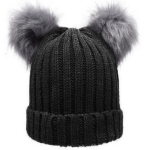
\includegraphics[height=1.5cm]{Images/Hats/winter}} & Kingsbury &
\begin{tabular}[c]{@{}l@{}} +2 Wisdom\\ +1 Charisma \\ +1 Constitution\end{tabular} &
  Sophie can can find it in Kingsbury near the main place or sew it in the magic castle. They are required grey wool threads x10 and grey
  fabric x4 & 4 \\\hline
  \textbf{Ascot cap} & \raisebox{-0.8\height}{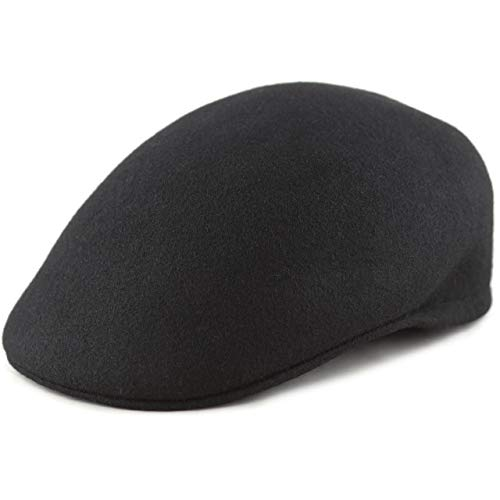
\includegraphics[height=1.5cm]{Images/Hats/ascotCap}} & Kingsbury &
  \begin{tabular}[c]{@{}l@{}}  -1 AC \\+1 Intelligence \\ +2 Constitution\end{tabular} & Sophie can can find it in
    Kingsbury in the eastern part of the city or sew it in the magic castle.  It is required leather x20 & 4 \\\hline            
    \textbf{Shako} & \raisebox{-0.8\height}{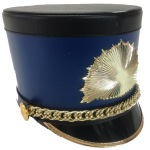
\includegraphics[height=1.5cm]{Images/Hats/shako}} & Dynamia &
    \begin{tabular}[c]{@{}l@{}} +2 Dexterity\\ -2 Intelligence\\ -1 Constitution \\+3 Strength\end{tabular} &
      Shako hat is a trophy that Sophie can get if she defeats 30 guards in Dynamia.& 4 \\\hline
      %\textbf{Turban} & \raisebox{-0.8\height}{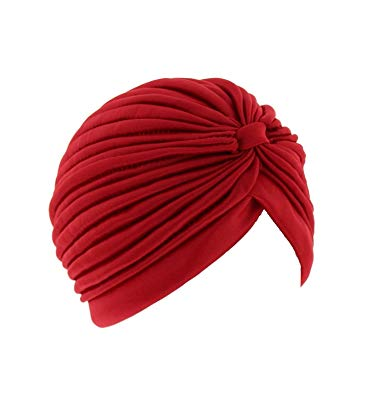
\includegraphics[height=1.5cm]{Images/Hats/turban}} & Dynamia
      %& \begin{tabular}[c]{@{}l@{}} +2 Dexterity \\ -2 TAC0 \end{tabular}  &
     % Sophie can find it in Dynamia it in the eastern part of the city. & 1 \\\hline
      \textbf{Baseball} & \raisebox{-0.8\height}{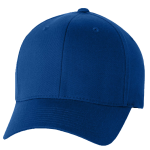
\includegraphics[height=1.5cm]{Images/Hats/baseball}} & Dynamia
      & \begin{tabular}[c]{@{}l@{}} +2 Constitution\\ +1 Wisdom\\ +2 Intelligence\end{tabular} &
          Sophie can buy it at the market of Dynamia for 250 coins. & 4\\\hline
          %\textbf{Chullo} & \raisebox{-0.8\height}{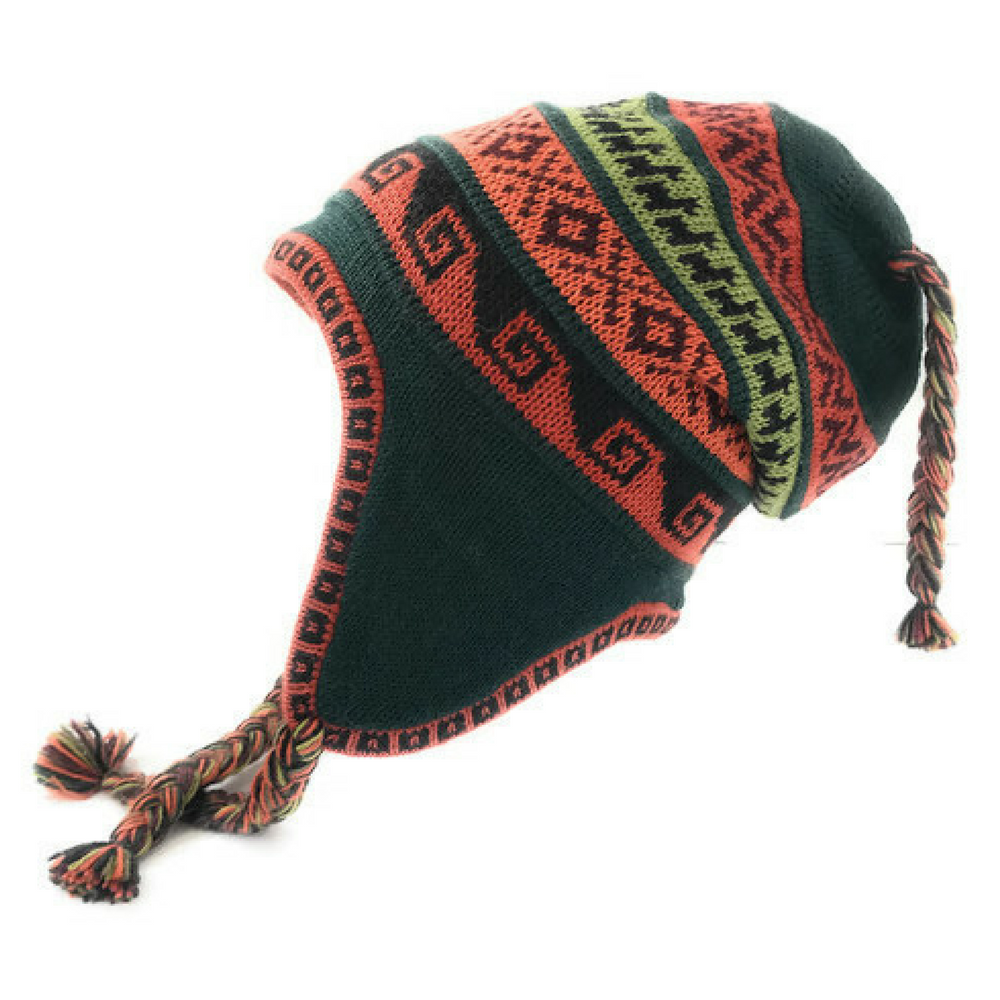
\includegraphics[height=1.5cm]{Images/Hats/chullo}} & Dynamia &
          %\begin{tabular}[c]{@{}l@{}}+2 Constitution\\ +2 Strength \\ -2 TAC0 \\ +3 HP\end{tabular} &
           % Sophie can buy it at the market of Dynamia for 350 coins. & 1 \\\hline
              \textbf{Nurse} & \raisebox{-0.8\height}{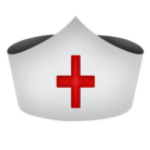
\includegraphics[height=1.5cm]{Images/Hats/nurse}} & Dynamia
              & \begin{tabular}[c]{@{}l@{}}+2 TAC0 \\ +3 Charisma\\ -3 Strength\\+2 Constitution\end{tabular} &
                  Sophie can get it if she plays a secundary mission. & 5 \\\hline
                  \textbf{Sombrero} & \raisebox{-0.8\height}{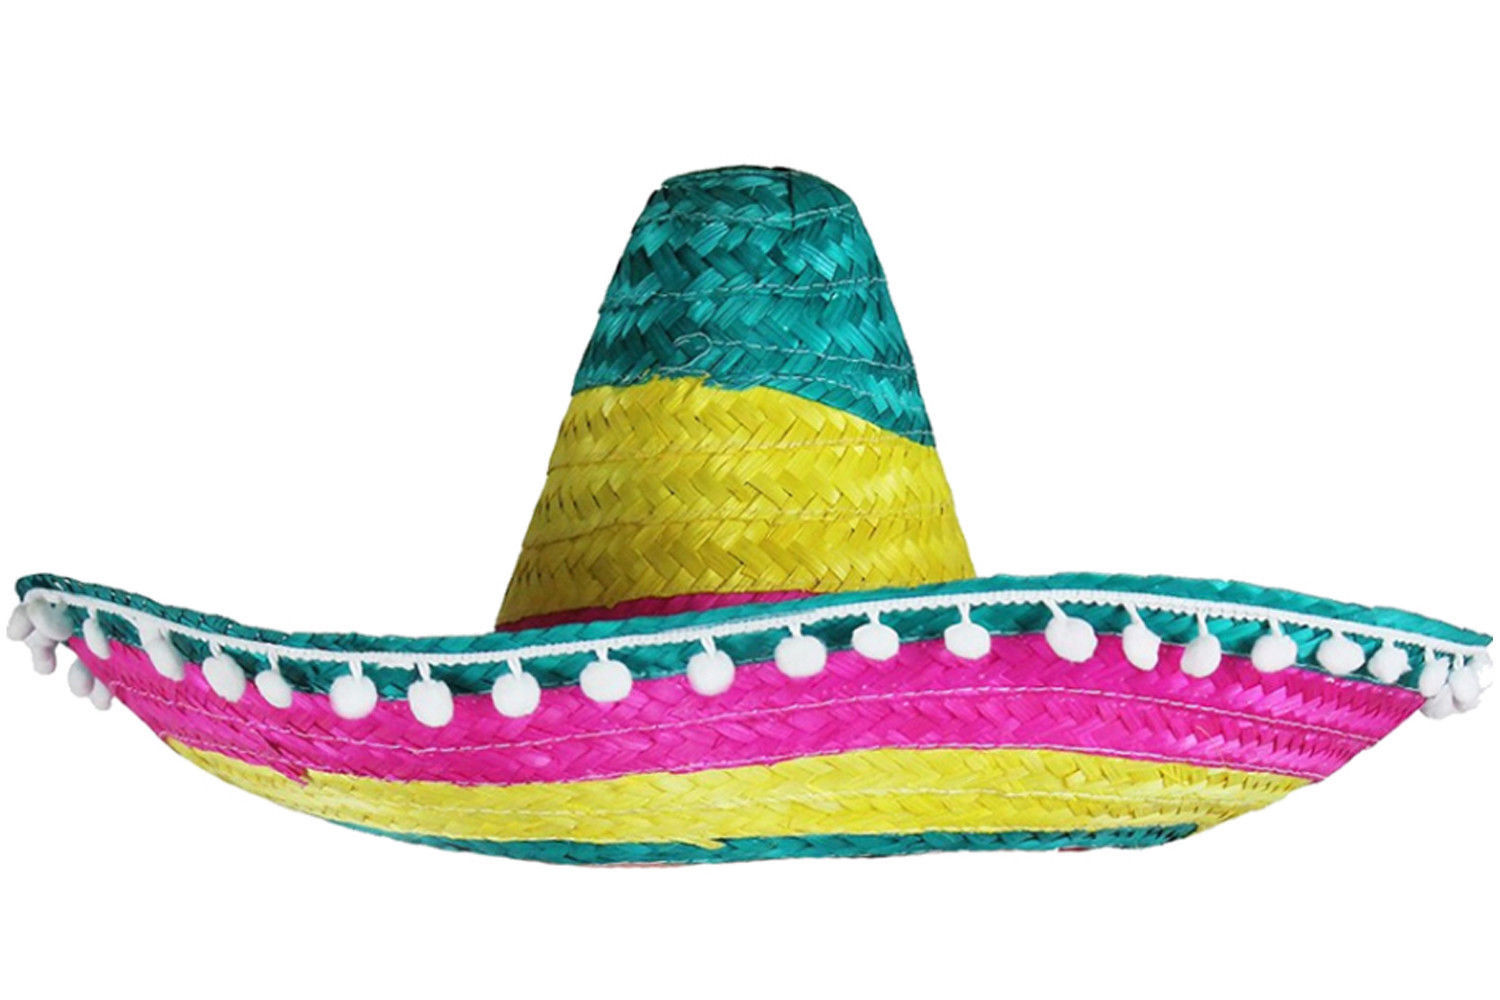
\includegraphics[height=1.5cm]{Images/Hats/sombrero}} & Flying castle
                  & +4 Constitution & Sophie can sew it in the magic castle. It is required 18 intelligence and three colored fabrics:
                  pink x1, yellow x2, light blue x3 & 4 \\\hline
                  \textbf{Bucket}  & \raisebox{-0.8\height}{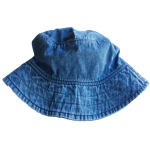
\includegraphics[height=1.5cm]{Images/Hats/bucket}}  & Flying castle
                  & \begin{tabular}[c]{@{}l@{}} +3 Charisma\\ -2 AC \\ +2 Strength\end{tabular} &
                      Sophie can sew it in the magic castle. It is required light blue fabric x6 & 4 \\\hline
                      \textbf{Fez} & \raisebox{-0.8\height}{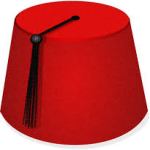
\includegraphics[height=1.5cm]{Images/Hats/fez}} & Flying castle
                      & \begin{tabular}[c]{@{}l@{}} +3 Charisma\\ -2 AC \\ +2 Dexterity \end{tabular} &
                          Sophie can sew it in the magic castle. It is required wool threads x20& 4 \\\hline
                          %\textbf{Capotain} & \raisebox{-0.8\height}{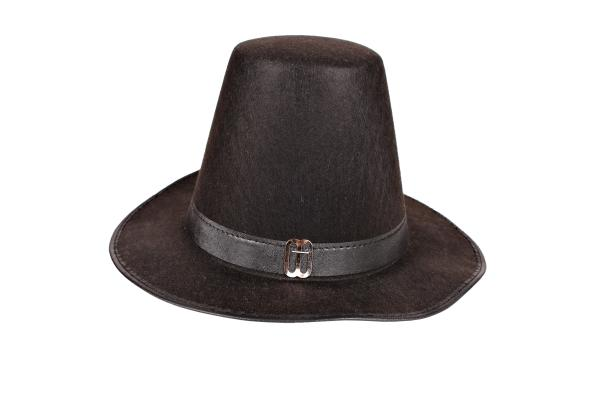
\includegraphics[height=1.5cm]{Images/Hats/capotain}}
                          %& Flying castle & \begin{tabular}[c]{@{}l@{}}+2 Constitution\\ +2 Strength \\ -2 TAC0 \\ +3 HP\end{tabular}
                           % & Sophie can sew it in the magic castle. They are required grey wool threads x5, leather x10 and grey
                            %fabric x5& 1 \\\hline
                            %\textbf{Winter red} & \raisebox{-0.8\height}{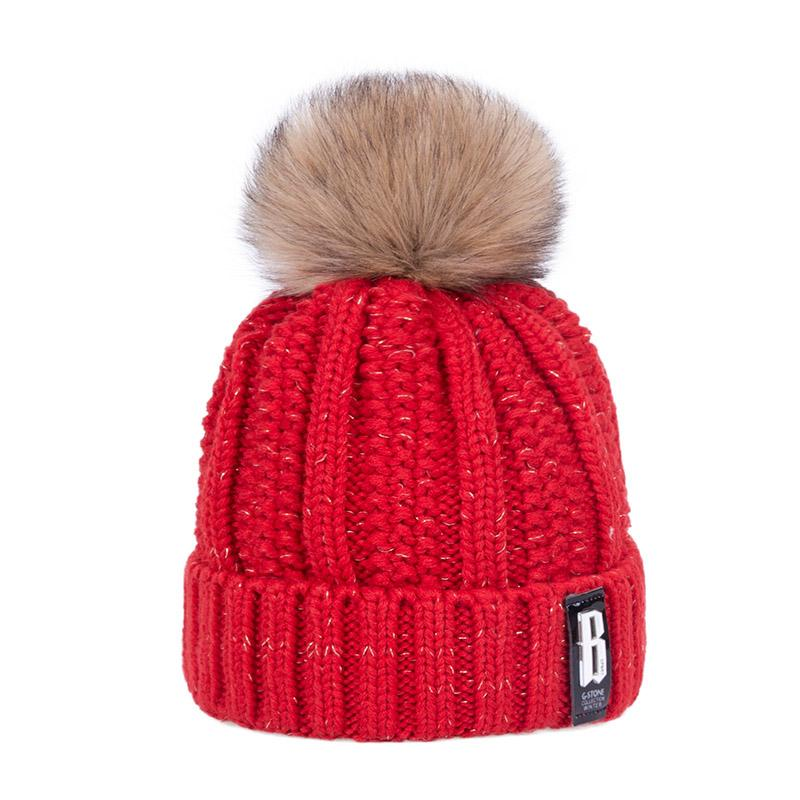
\includegraphics[height=1.5cm]{Images/Hats/winterRed}}
                            %& Flying castle   &\begin{tabular}[c]{@{}l@{}} +2 Wisdom\\ +2 HP\end{tabular} & Sophie can sew it in the magic castle. They are required red wool threads x10 and red fabric x4 & 1 \\\hline
\textbf{Christmas}& \raisebox{-0.8\height}{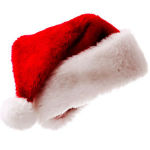
\includegraphics[height=1.5cm]{Images/Hats/christmas}} & Flying castle & \begin{tabular}[c]{@{}l@{}}+4 Wisdom\\ +2 Strength \\ -2 TAC0 \\ +2 Constitution\end{tabular} & Sophie can sew it in the magic castle. They are required white wool threads x12 and red fabric x6& 4 \\\hline
%\textbf{Crest} & \raisebox{-0.8\height}{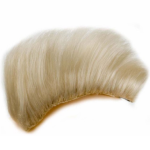
\includegraphics[height=1.5cm]{Images/Hats/crest}}                & Flying castle                                                  &\begin{tabular}[c]{@{}l@{}} +2 Strength\\ -4 Intelligence\\ -1 HP\end{tabular} & Sophie can sew it in the magic castle. It is required white and/or yellow wool threads x30 & 1 \\\hline
\textbf{Non la}                      & \raisebox{-0.8\height}{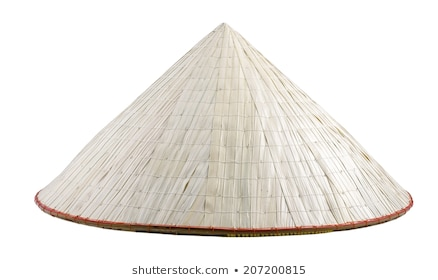
\includegraphics[height=1.5cm]{Images/Hats/nonLa}}             & Flying castle                                                  & \begin{tabular}[c]{@{}l@{}}+3 Intelligence\\ +3 Wisdom\\ -3 Strength\end{tabular}     & Sophie can sew it in the magic castle. They are required straw x20 and leather x5                                                      & 4 \\\hline
%\textbf{Airplane}                  & \raisebox{-0.8\height}{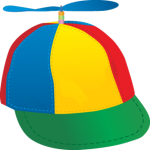
\includegraphics[height=1.5cm]{Images/Hats/airplane}}          & Flying castle                                                  & \begin{tabular}[c]{@{}l@{}}+3 Charisma\\ +10 HP\\ -3 Strength\end{tabular} & Sophie can sew it in the magic castle. It is required wool threads x20                                                           & 1 \\\hline
%\textbf{Jewish}                      & \raisebox{-0.8\height}{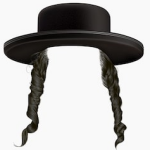
\includegraphics[height=1.5cm]{Images/Hats/jewish}}             & Flying castle                                                  & \begin{tabular}[c]{@{}l@{}} +2 Strength\\ -4 Intelligence\\ -1 HP\end{tabular} & Sophie can sew it in the magic castle. They are required black wool threads x20 and leather x20                                        & 1 \\\hline
\textbf{Boomers helmet}              & \raisebox{-0.8\height}{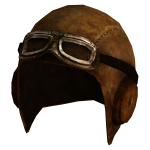
\includegraphics[height=1.5cm]{Images/Hats/boomersHelmet}}      & Everywhere                                                     & \begin{tabular}[c]{@{}l@{}}+4 Dexterity\\ +4 Charisma\\ +2 TAC0\end{tabular}            & Boomers helmet is a trophy that Sophie can get flying with the castle over 100kms.                                                     & 7 \\\hline
\textbf{Bearskin}                    & \raisebox{-0.8\height}{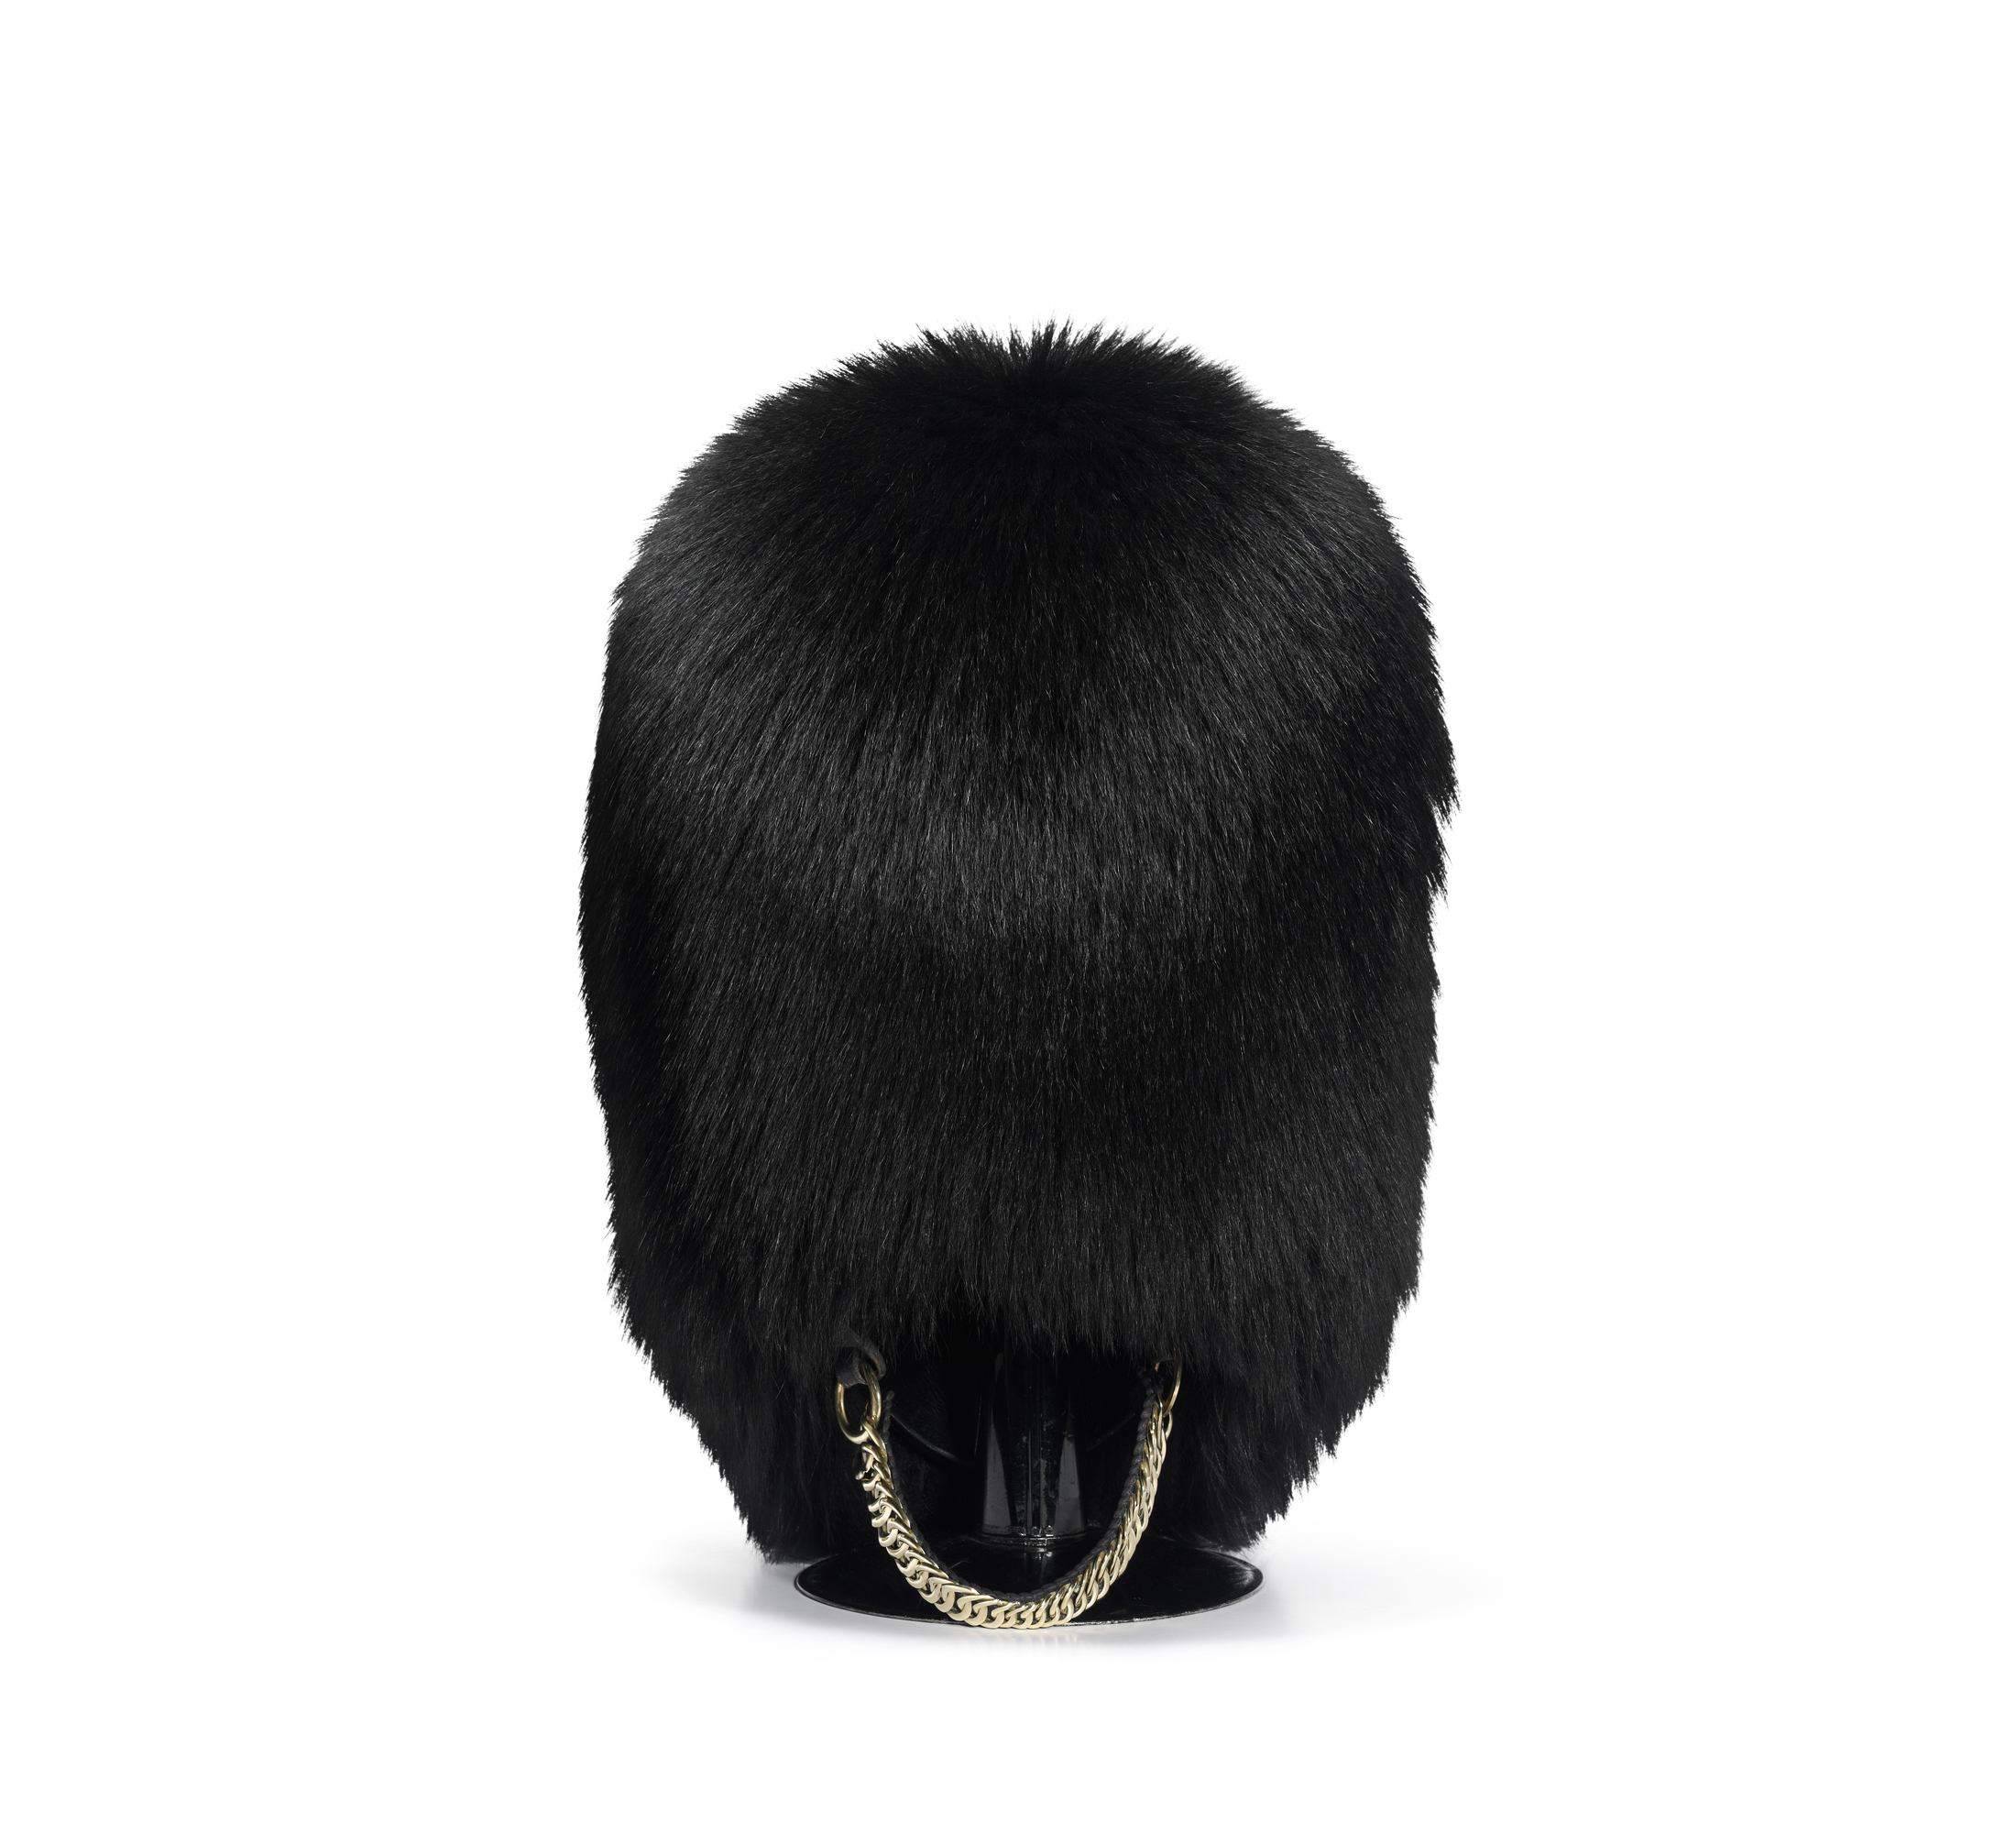
\includegraphics[height=1.5cm]{Images/Hats/bearskin}}           & Desert                                                      & \begin{tabular}[c]{@{}l@{}}+4 Charisma\\ -1 TAC0 \\ +4 Strength\end{tabular} & Bearskin is a trophy that Sophie can get if she sees 40 guards in Kingsbury.                                                           & 6 \\\hline
%\textbf{Magic} & \raisebox{-0.8\height}{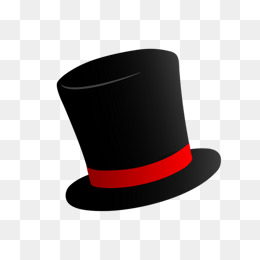
\includegraphics[height=1.5cm]{Images/Hats/magic}} & Everywhere & \begin{tabular}[c]{@{}l@{}} +2 Wisdom\\ +2 HP\end{tabular}  & Magic is a trophy that Sophie gets if she talks with 50 objects.                                                                    & 1 \\\hline
%\textbf{Malefica} & \raisebox{-0.8\height}{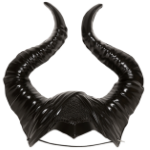
\includegraphics[height=1.5cm]{Images/Hats/malefica}} & Southern desert  & \begin{tabular}[c]{@{}l@{}} +2 Strength\\ -4 Intelligence\\ -1 HP\end{tabular} & Sophie receives it if she finds 1 other collectable in the desert & 1 \\\hline
\textbf{Mask}                           & \raisebox{-0.8\height}{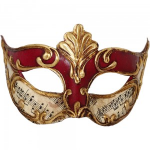
\includegraphics[height=1.5cm]{Images/Hats/mask}}              & Southern desert   & \begin{tabular}[c]{@{}l@{}}+4 Charisma\\ +4 Wisdom\\ +3 Intelligence\end{tabular} & Sophie gets it if she finds 3 other collectables in the desert & 6 \\\hline
\textbf{Bear headgear}                           & \raisebox{-0.8\height}{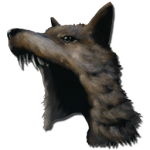
\includegraphics[height=1.5cm]{Images/Hats/headgear}}              & Spirits realm & \begin{tabular}[c]{@{}l@{}} +5 TAC0\\ +1 Charisma \\ -4 AC\end{tabular} & Sophie gets it if she walks for 3 km& 4 \\\hline
\textbf{Dog headgear}                           & \raisebox{-0.8\height}{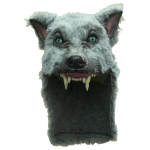
\includegraphics[height=1.5cm]{Images/Hats/headgear1}}              & Spirits realm  & \begin{tabular}[c]{@{}l@{}} +3 Strength\\ +4 Intelligence\\ +4 Charisma\\-1 Constitution\end{tabular} & This headgear is hidden int the spirits realm & 8 \\\hline
\textbf{Helmet}& \raisebox{-0.8\height}{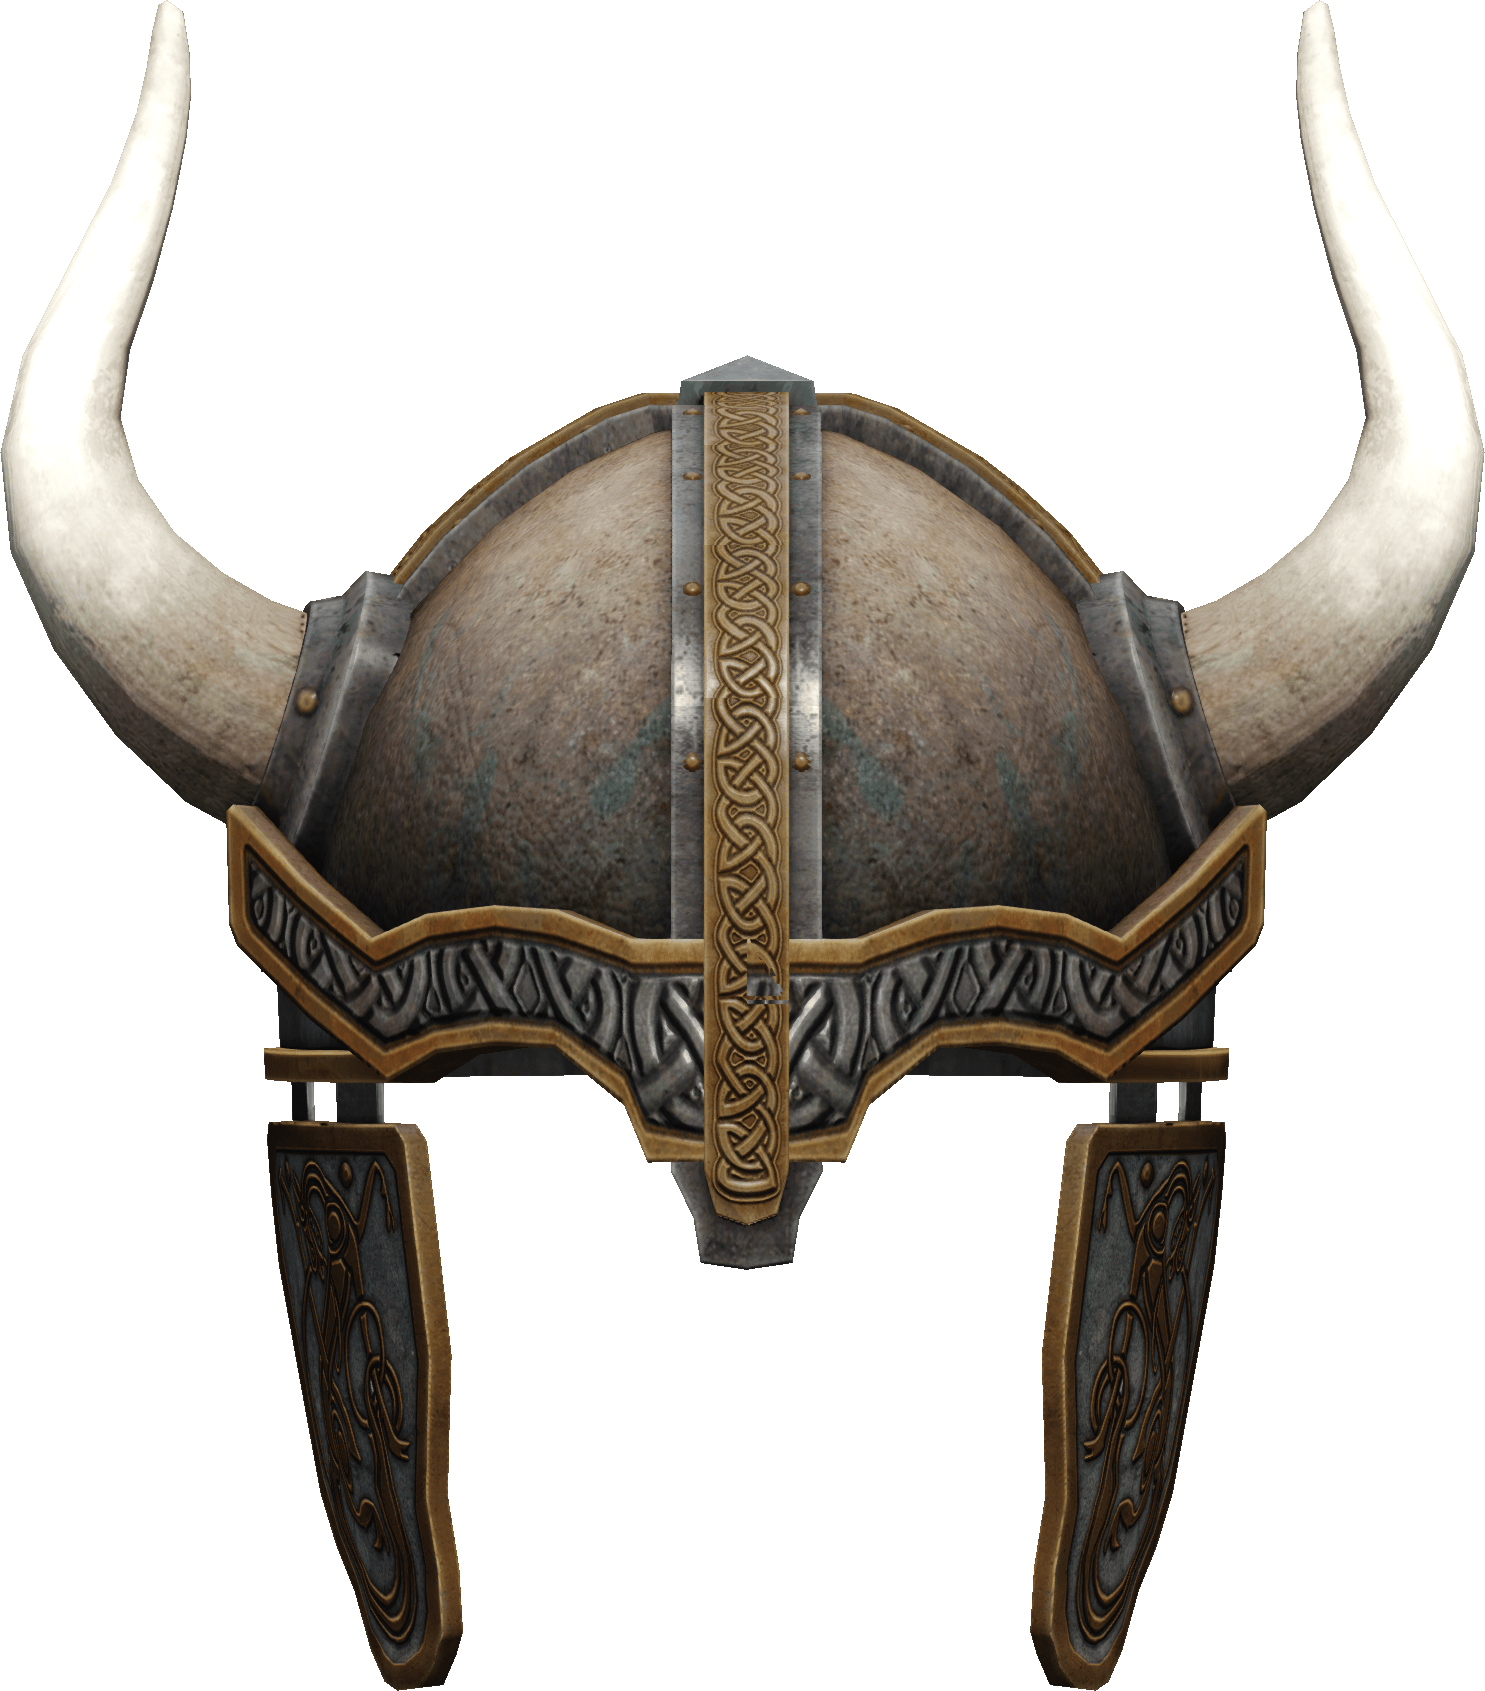
\includegraphics[height=1.5cm]{Images/Hats/helmet}} & Kazan island &
            \begin{tabular}[c]{@{}l@{}} +4 TAC0 \\ +3 Dexterity\\ +2 Strength\\ +6 Constitution \\ -2 AC\end{tabular} &
              Sophie may get it speaking with an hidden object & 7 \\\hline
%\textbf{Pungiball}                           & \raisebox{-0.8\height}{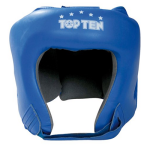
\includegraphics[height=1.5cm]{Images/Hats/headgear3}}              & Spirits realm  & \begin{tabular}[c]{@{}l@{}}+2 Constitution\\ +2 Strength \\ -2 TAC0 \\ +3 HP\end{tabular} & Pungiball is a trophy that Sophie gets if she runs over 5kms. & 1 \\\hline
\textbf{American}                           & \raisebox{-0.8\height}{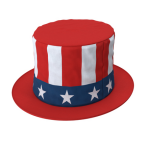
\includegraphics[height=1.5cm]{Images/Hats/american}}              & Kazan island & \begin{tabular}[c]{@{}l@{}} +6 TAC0\\ +2 Constitution \\ +3 Wisdom \\ +4 Dexterity \\ +3 Intelligence \\ +2 Strength\end{tabular} & Sophie gets it if she plays both the endings of the game & 9 \\\hline
\end{longtable}

}

\item \textbf{Lanterns}\\
  {\small
\begin{longtable}[H]{|p{1.8cm}|p{1.5cm}|p{2cm}|p{2.6cm}|p{5.3cm}|p{1.2cm}|}

      \hline
      \multicolumn{6}{|c|}{\cellcolor[HTML]{656565}{\color[HTML]{FFFFFF} \textbf{Collectable}}}                                                                                                                                                                                                                                                                                                                                     \\ \hline
      \multicolumn{1}{c|}{\cellcolor[HTML]{C0C0C0}\textbf{Hats}} & \cellcolor[HTML]{C0C0C0}{\color[HTML]{000000} \textbf{Image}}
      & \multicolumn{1}{c|}{\cellcolor[HTML]{C0C0C0}{\color[HTML]{000000} \textbf{Location}}} &
      \multicolumn{1}{c|}{\cellcolor[HTML]{C0C0C0}{\color[HTML]{000000} \textbf{Bonus}}} &
      \multicolumn{1}{c|}{\cellcolor[HTML]{C0C0C0}{\color[HTML]{000000} \textbf{Brief description}}} &
       \multicolumn{1}{c|}{\cellcolor[HTML]{C0C0C0}{\color[HTML]{000000} \textbf{Difficulty}}} \\\hline
  \textbf{Spacious} & \multicolumn{1}{c|}{\raisebox{-0.8\height}{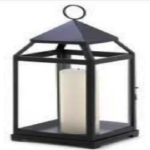
\includegraphics[height=1.5cm]{Images/Lanterns/spacious}}} &
  Everywhere & \begin{tabular}[c]{@{}l@{}} 1d8 \\ +1 Strength \\ +1 Intelligence \end{tabular} & Sophie get it defeating 10 enemies or
  solving 10 puzzles & 4\\ \hline
  \textbf{Smelly} & \raisebox{-0.8\height}{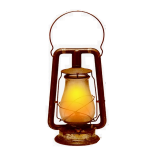
\includegraphics[height=1.5cm]{Images/Lanterns/smelly}} & Dynamia &
  \begin{tabular}[c]{@{}l@{}} 1d8 \\ +2 Strength \\ +5 HP \end{tabular} & Sophie can find it in the southern part of the city & 7\\ \hline
  \textbf{Perfumed} & \raisebox{-0.8\height}{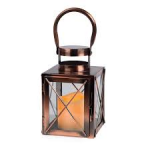
\includegraphics[height=1.5cm]{Images/Lanterns/perfumed}} &  Dynamia  &
  \begin{tabular}[c]{@{}l@{}} 1d8 \\ +3 TAC0  \end{tabular} & Sophie can find it in the western part of
  the city & 7\\ \hline
  \textbf{Silver} & \raisebox{-0.8\height}{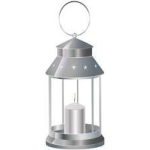
\includegraphics[height=1.5cm]{Images/Lanterns/silver}} & Kingsbury  &
  \begin{tabular}[c]{@{}l@{}} 1d10 \\ -2 Strength \\ +1 Wisdom \\ +5 HP \end{tabular} & Sophie can find it near the castle & 3\\ \hline
  \textbf{Diamonds} & \raisebox{-0.8\height}{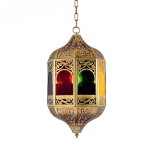
\includegraphics[height=1.5cm]{Images/Lanterns/diamonds}} & Kingsbury &
  \begin{tabular}[c]{@{}l@{}} 1d6 \\ +5 Strength \\ -2 AC \\ +5 HP \end{tabular} & Sophie get it defeating 65 enemies & 4\\ \hline
  \textbf{China} & \raisebox{-0.8\height}{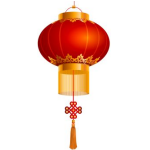
\includegraphics[height=1.5cm]{Images/Lanterns/china}} & Southern Desert &
  \begin{tabular}[c]{@{}l@{}} 1d6 \\ +3 Strength \\ -1 AC \\ +4 Dexterity \\ + HP \end{tabular} &
  Sophie gets it if she wander for 30km in Southern Desert & 5 \\ \hline
  \textbf{One hit} & \raisebox{-0.8\height}{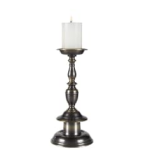
\includegraphics[height=1.5cm]{Images/Lanterns/candelabrum}} & Everywhere &
  \begin{tabular}[c]{@{}l@{}} 2d10 \\ +3 Strength \\ +4 AC \\ -2 Intelligence \end{tabular} &
  Sophie gets it when she will have got all other lanterns & 9\\ \hline
  \textbf{Arabic} & \raisebox{-0.8\height}{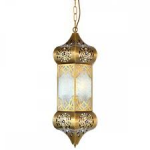
\includegraphics[height=1.5cm]{Images/Lanterns/arabic}} & Southern Desert &
  \begin{tabular}[c]{@{}l@{}} 1d8 \\+3 Strength \\+10 HP \end{tabular} & Sophie gets it if she wander for 50km in Southern Desert & 8\\ \hline
\end{longtable}
}

\item \textbf{Clothes}\\
  \begin{longtable}[H]{|p{2cm}|p{1.5cm}|p{2cm}|p{2.8cm}|p{6.3cm}|}
  \hline
  \multicolumn{1}{c|}{\cellcolor[HTML]{C0C0C0}\textbf{Clothes}} & \cellcolor[HTML]{C0C0C0}{\color[HTML]{000000} \textbf{Image}} & \multicolumn{1}{c|}{\cellcolor[HTML]{C0C0C0}\textbf{Location}} & \multicolumn{1}{c|}{\cellcolor[HTML]{C0C0C0}{\color[HTML]{000000} \textbf{Bonus}}}    & \multicolumn{1}{c|}{\cellcolor[HTML]{C0C0C0}{\color[HTML]{000000} \textbf{Brief description}}}                                         \\ \hline
\textbf{I Love Venice}& \raisebox{-0.8\height}{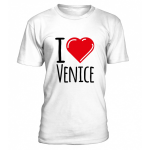
\includegraphics[height=1.5cm]{Images/Clothes/iLoveVenice}} & Dynamia & TODO
& Sophie can get it in Dynamia. It is placed in a hiding place that can be reached at any time during the game.\\ \hline
\end{longtable}


\end{enumerate}


